The breast cancer dataset was the second mandatory dataset. We got a score of 97.647\% on kaggle.

\subsection{Characteristics}

\begin{itemize}
\item No missing values
\item binary target class (B and M)
\item Only rational features
\item 30 attributes (disregarding id)
\item 285 samples
\end{itemize}


\subsection{Characteristics of Classifiers}

There are two target classes, B and M. While 96 of the samples are of type M, 189 are of type M. As there are more in type M, samples that are not easily seperable might lead to worse results.

\begin{figure}[H]
  \begin{center}
    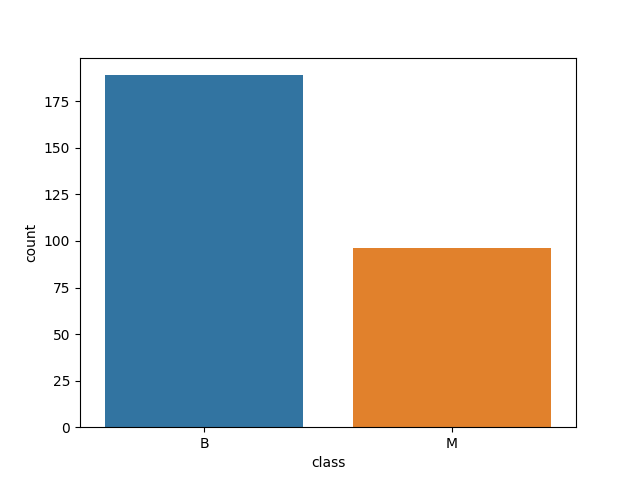
\includegraphics[width=0.8\linewidth]{breast/plots/countplot.png}
    \caption{Histogram of the target values}
    \label{fig:breast-target}
  \end{center}
\end{figure}

\subsection{Feature Selection}
First different plots to visualize the data were made. The results can be seen in Figure \ref{fig:breast-vionline1}

\begin{figure}[H]
  \begin{center}
    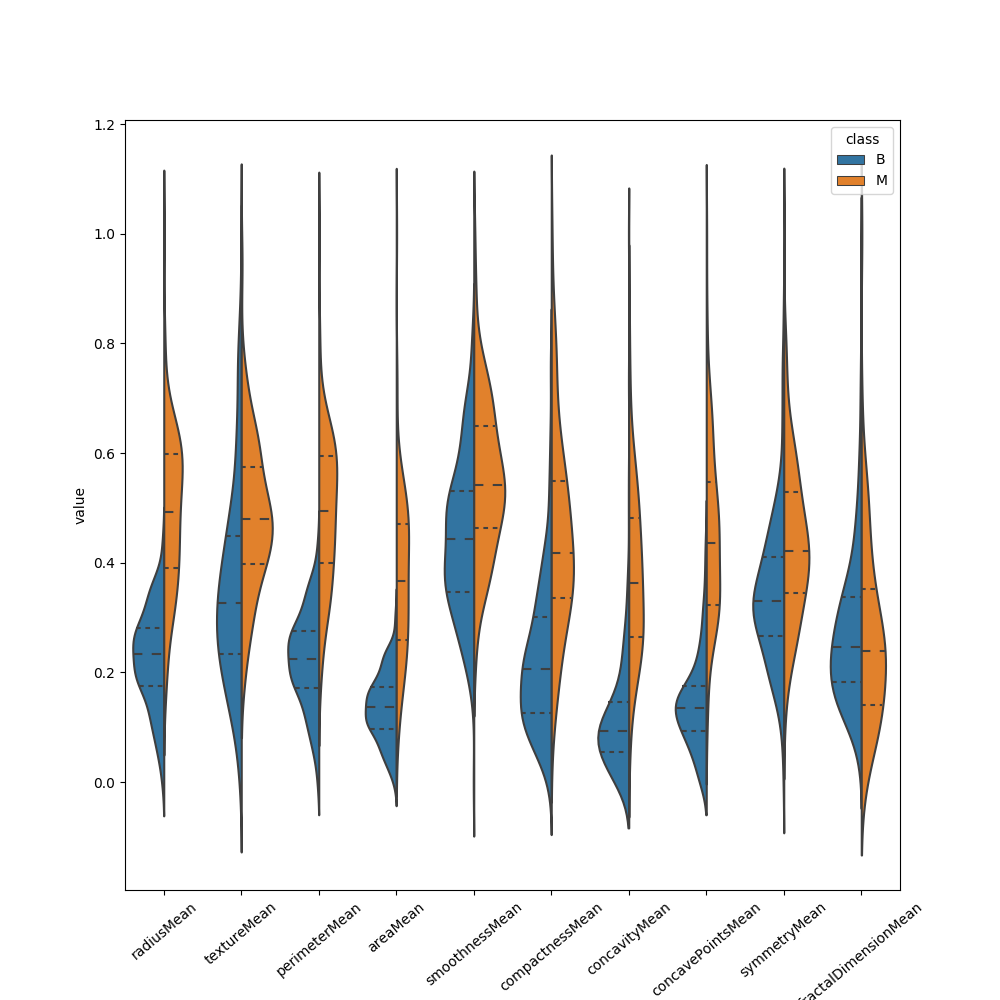
\includegraphics[width=0.8\linewidth]{breast/plots/violinplot.png}
    \caption{Histogram of the target values}
    \label{fig:breast-vionline1}
  \end{center}
\end{figure}

\subsection{K Nearest Neighbors Classifier}



As seen in Figure \ref{fig:breast-knn-metrics} euclidean works best as a metric.

\begin{figure}[H]
  \begin{center}
    \includegraphics[width=0.8\linewidth]{breast/plots/knn_p_comparison.png}
    \caption{Histogram of the target values}
    \label{fig:breast-knn-metrics}
  \end{center}
\end{figure}

As seen in Figure \ref{fig:breast-knn-comparison} preprocessing is actually worse than without preprocessing.

\begin{figure}[H]
  \begin{center}
    \includegraphics[width=0.8\linewidth]{breast/plots/knn_feature_comparison.png}
    \caption{Histogram of the target values}
    \label{fig:breast-knn-comparison}
  \end{center}
\end{figure}

\subsection{Random Forest Classifier}

\ref{fig:breast-rf-comparison}

\begin{figure}[H]
  \begin{center}
    \includegraphics[width=0.8\linewidth]{breast/plots/knn_feature_comparison.png}
    \caption{Histogram of the target values}
    \label{fig:breast-rf-comparison}
  \end{center}
\end{figure}

\subsection{Multi-Layer Perceptron Classifier}

\subsection{Conclusion}

